%template1.tex
%The following LaTeX source file represents the simplest kind of slide presentation; no overlays, no included graphics. Substitute your favorite style for ``pascal''. To create the PDF file template1.pdf, (1) be sure to use the prosper class, then (2) execute the command latex template1.tex, and (3) the command dvipdf template1.dvi.

%%%%%%%%%%%%%%%%%%%%%%%%%%%%%%% template1.tex %%%%%%%%%%%%%%%%%%%%%%%%%%%%%%%%%%%
\documentclass[a4paper,blends,pdf,colorBG,slideColor]{prosper}
% definitions for slides for CSC544
% Lutz Hamel, (c) 2007

\hypersetup{pdfpagemode=FullScreen}

\usepackage{times}
\usepackage{latexsym}
\usepackage{alltt}
\usepackage{booktabs}
\usepackage{amsmath}
\usepackage{amsopn}
\usepackage{amsfonts}
\usepackage{amssymb}
%\usepackage[usenames]{color}

\def\sign{\qopname\relax{no}{sign}}
\def\argmax{\qopname\relax{no}{argmax}}
\def\argmin{\qopname\relax{no}{argmin}}

\newcommand{\grad}{\ensuremath{\nabla}} 
\newcommand{\loss}{\ensuremath{{\cal L}}}
\newcommand{\err}{\mbox{err}}
\newcommand{\mse}{\mbox{mse}}
\newcommand{\acc}{\mbox{acc}}
\newcommand{\Integer}{\ensuremath{\mathbb{N}}}
\newcommand{\size}[1]{{|{#1}|}}
\newcommand{\Rnspace}[1]{\ensuremath{\mathbb{R}^{#1}}}
\newcommand{\Real}{\ensuremath{\mathbb{R}}}
\newcommand{\mytt}[1]{{\small\tt{#1}}}
\newcommand{\textemph}[1]{{\em #1}}
\newcommand{\suchthat}{\mid}
\newcommand{\orbar}{\;|\;}
\newcommand{\bs}[1]{\begin{slide}{#1}\ptsize{8}}
\newcommand{\es}{\end{slide}}
\newcommand{\co}{\,\colon\;}
\newcommand{\pair}[2]{\ensuremath{( {#1}, {#2} )}}
\newcommand{\model}[1]{\hat{#1}}
\newcommand{\ul}[1]{{\bf\em #1}}
\newcommand{\ol}{\overline}
\newcommand{\definition}[1]{{\bf Definition: }{\em #1}}
\newcommand{\example}[1]{{\bf Example: }{#1}}
\newcommand{\abs}[1]{|{#1}|}
\newcommand{\mytab}{\makebox[.1in]{}}

\newcommand{\fdef}[1]{
\begin{center}
\fbox{
\begin{minipage}{3.5in}
{\bf Definition:}
{#1}
\end{minipage}
}
\end{center}
}

\newcommand{\fframe}[1]{
\begin{center}
\fbox{
\begin{minipage}{3.5in}
{#1}
\end{minipage}
}
\end{center}
}

\newcommand{\nframe}[1]{
\begin{center}
\begin{minipage}{3.5in}
{#1}
\end{minipage}
\end{center}
}

\newenvironment{Rcode}
	{
		\scriptsize
		\begin{quote}
		\begin{alltt}
	}
	{
		\end{alltt}
		\end{quote}
	}




\begin{document}

\bs{Regression as Machine Learning}
Given
\begin{itemize}
\item A data universe $X$.
\item A sample set $S$ where $S \subset X$.
\item Some target function $f\co X \rightarrow {\color{red}\Real}$.
\item A training set $D$, where
$
D = \{ (x ,y) \suchthat x \in S \text{ and } y = f(x)\}.
$
\end{itemize}
Compute a model $\model{f}\co X \rightarrow {\color{red}\Real}$ using $D$ such that,
\begin{equation*}
\model{f}(x) \cong f(x),
\end{equation*}
for all $x \in X$.

\vspace{.1in}

{\bf Observation:}  Same as machine learning in classification except for the co-domains 
of the target function and the model.

{\bf Question:} How do we compute the model?

\es


\bs{Regression ANNs}
The perceptron revisited
\begin{center}
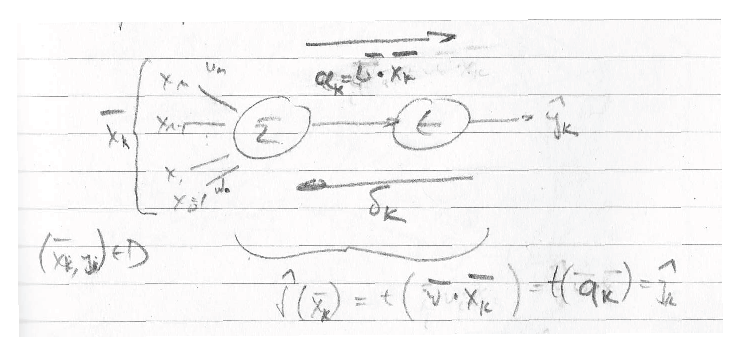
\includegraphics[height=30mm]{images/perceptron-revisited.eps}
\end{center}
\es

\bs{Regression ANNs}
Recall
\begin{eqnarray*}
E_k(\ol{w}) &=& \frac{1}{2}(y_k - \model{y}_k)^2\\
	&=& \frac{1}{2}(y_k-t(\ol{w}\bullet\ol{x}_k)^2\\
	&=& \frac{1}{2}(y_k-t(a_k))^2
\end{eqnarray*}

Learning defined in terms of numerical error instead of classification error - regression by default!

We turn the regression problem into a classification problem by applying {\em thresholding}.
\es

\bs{Regression ANNs}
We can now look at the gradient,
\begin{eqnarray*}
\grad E_k(\ol{w}) &=& \frac{d}{d\ol{w}} E_k(\ol{w}) \\
	&=& \frac{1}{2} \frac{d}{d\ol{w}}(y_k-t(a_k))^2\\
	&=& -(y_k -t(a_k))\frac{dt}{d\ol{w}}(a_k)\\
	&=& -(y_k -\model{y}_k)\frac{dt}{d\ol{w}}(a_k)\\
	&=& -(y_k -\model{y}_k)\frac{dt}{da_k} (a_k) \frac{da_k}{d\ol{w}} \mbox{ (chain rule)}\\
	&=& -(y_k -\model{y}_k)t'(a_k) \frac{d}{d\ol{w}}(\ol{w}\bullet\ol{x}_k) \\
	&=& -(y_k -\model{y}_k)t'(a_k) \ol{x}_k \\
	&=& \delta_k \ol{x}_k
\end{eqnarray*}
where $\delta_k = -(y_k -\model{y}_k)t'(a_k)$ is called the error.
\es


\bs{Regression ANNs}
Now recall our update rule,
\[
\ol{w} \leftarrow \ol{w} + \Delta \ol{w}
\]
From before we have
\[
\ol{w} \leftarrow \ol{w} + \eta \grad E_k(\ol{w})
\]
From our discussion above it follows that
\[
\ol{w} \leftarrow \ol{w} + \eta \delta_k\ol{x}_k
\]

\vspace{.2in}
{\bf Observation:} The weights are updated using a scaled version of the input vector.  It is also easy to see that the weights are scaled 
proportional to the error.

This is called {\em back propagation.}

If we can take the derivative of the transfer function then we can easily extend this to multi-layer neural networks.
\es

\end{document}
%%%%%%%%%%%%%%%%%%%%%%%%%%% end of template1.tex %%%%%%%%%%%%%%%%%%%%%%%%%%%%%%%%

